\chapter{Progettazione e codifica}
\label{chap:progettazione}

\section{Strumenti di supporto}
Di seguito vengono descriti alcuni degli strumenti di supporto utilizzati per la progettazione e lo sviluppo del software. Il primo è lo strumento utilizzato per la scrittura vera propria del codice, a seguire il \textit{tool} per gestire la continua evoluzione di esso, l'ultimo per la creazione e per il \textit{testing} delle \gls{API}.

\subsection{Spring Tools}

\begin{figure}
\begin{center}

\includegraphics[width=0.7\columnwidth]{images/springtoollogo2.png}
\end{center}
\caption{Logo Spring Tools}
\label{fig:stslogo}
\end{figure}

Spring Tool Suite è un ambiente di sviluppo integrato, derivato dall'\gls{IDE} Eclipse. Permette uno sviluppo più veloce di applicativi basati su Spring. Fornisce supporto al linguaggio Java, al \gls{framework} Spring ed all'eventuale ambiente di sviluppo \cite{springtool}. 






\subsection{GitLab}
\begin{figure}
\begin{center}

\includegraphics[width=0.4\columnwidth]{images/GitLab_logo.png}
\end{center}
\caption{Logo GitLab}
\label{fig:gitlab}
\end{figure}


GitLab è un software per il controllo di versione, esso permette la creazione di \gls{repository} pubblici o privati, in cui gli sviluppatori possono caricare il proprio codice e gestire le modifiche alle varie versioni in contemporanea al lavoro di più persone \cite{gitlab}.

\subsection{Postman}
\begin{figure}
\begin{center}

\includegraphics[width=1.0\columnwidth]{images/postmanlogo.png}
\end{center}
\caption{Logo Postman}
\label{fig:postman}
\end{figure}


Postman è un ambiente di sviluppo che aiuta gli sviluppatori a creare, testare, documentare, monitorare e pubblicare documentazione per le loro \gls{API} \cite{postman}. Le caratteristiche principali di questo strumento sono: \cite{postmaninfo}
\begin{itemize}
    \item invio di richieste \gls{API}.
    \item \gls{debugging} e salvataggio delle risposte.
    \item organizzazione delle \gls{API} in gruppi denominati Raccolte.
    \item condivisione e collaborazione delle raccolte con il team. 
\end{itemize}
\section{Progettazione}
Nel corso dello sviluppo dell'applicazione il team ha sviluppato l'architettura del progetto cercando di mantenerla il più semplice e lineare possibile. Il risultato della progettazione è un 'architettura \textit{multi-tier}, ovvero un'architettura software di tipo \textit{client-server} in cui le varie funzionalità del software sono logicamente separate ovvero suddivise su più strati o livelli software differenti in comunicazione tra loro \cite{multitier}.\\
L'architettura progettata si presenta suddivisa in cinque strati: 

\begin{itemize}
    \item front-end
    \item \gls{API}
    \item logica di \textit{business}
    \item integrazione
    \item \gls{DAO}
\end{itemize}
\clearpage


Nell'immagine sottostante (\ref{fig:archisw}) si cerca di dare una visione grafica dell'architettura progettata da parte del team e la comunicazione che avviene tra i vari livelli.


\begin{figure}
\begin{center}
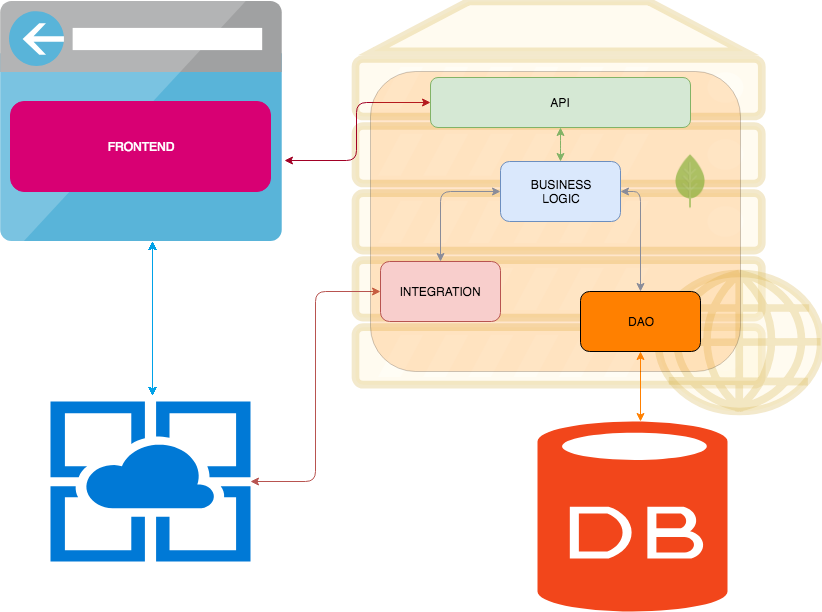
\includegraphics[width=0.8\columnwidth]{images/architetturasw.png}
\end{center}
\caption{Architettura software Web Application \cite{archiprog}}
\label{fig:archisw}
\end{figure}

\subsection{Front-end}
Tutti gli \gls{URL} navigabili tramite l'applicazione vengono riportati qui di seguito:

\begin{itemize}
    \item \textbf{/ :} è la pagina principale, avviata al momento dell’applicazione. Sebbene
sia navigabile, non esiste realmente. L’utente viene infatti immediatamente
reindirizzato a \textbf{/home};
    \item \textbf{/home:} è la vera pagina principale, nella quale vengono mostrate le possibili attività da svolgere nell'applicazione; 
    \item \textbf{/login:} è la pagina nella quale l'utente registrato può effettuare il login con le sue credenziali;
    \item \textbf{/user\_management:} è la pagina nella quale l'amministratore può gestire le altre utenze;
    \item \textbf{/new\_flow:} è la pagina nella quale l'utente può creare un nuovo flusso logico;
    \item \textbf{/flow\_management:} è la pagina nella quale l'utente può ricercare, visualizzare, modificare ed eliminare flussi già esistenti;
    \item \textbf{**:} è una qualunque altra pagina che l'utente può digitare, verrà poi automaticamente reindirizzato verso la pagina \textbf{/error};
    \item \textbf{/error:} è la pagina di errore che viene visualizzata in caso di errori o di richieste da parte dell'utente non gestite dall'applicazione;
\end{itemize}


\begin{figure}
\begin{center}
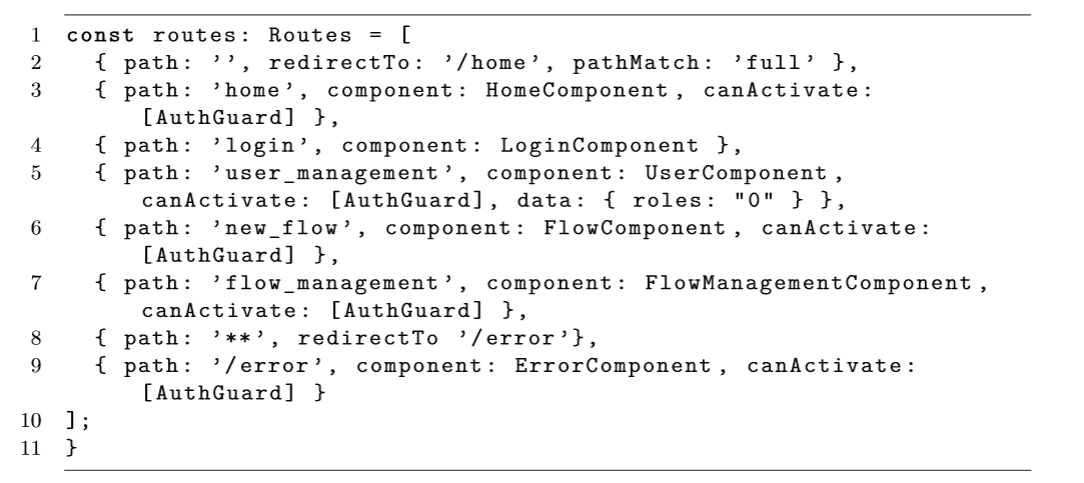
\includegraphics[width=1.0\columnwidth]{images/router.png}
\end{center}
\caption{File di configurazione del componente \textit{router}}
\label{fig:router}
\end{figure}
% \begin{lstlisting}[language=Java, label=lst:router, caption={}]
% const routes: Routes = [
%   { path: '', redirectTo: '/home', pathMatch: 'full' },
%   { path: 'home', component: HomeComponent, canActivate: [AuthGuard] },
%   { path: 'login', component: LoginComponent },
%   { path: 'user_management', component: UserComponent, canActivate: [AuthGuard], data: { roles: "0" } },
%   { path: 'new_flow', component: FlowComponent, canActivate: [AuthGuard] },
%   { path: 'flow_management', component: FlowManagementComponent, canActivate: [AuthGuard] },
%   { path: '**', redirectTo '/error'},
%   { path: '/error', component: ErrorComponent, canActivate: [AuthGuard] }
% ];
% }
% \end{lstlisting}









\subsection{Back-end}

\subsubsection{End-point}
Di seguito verranno riportati gli \textit{end-points}, ovvero le \gls{API} \gls{HTTP} messe a disposizione dal \textit{back-end} per essere \textit{consumate} dal \textit{front-end}. Le \gls{API} sono raggruppate sulla base del servizio nel quale operano e per il metodo \gls{HTTP} (GET, POST, PUT e DELETE) utilizzato.\\
\ \\
\textbf{\textit{User Service}}
\begin{itemize}
    \item PUT /users/\{id\}: utilizzata per la modifica di un utente esistente dato l'id.
    \item DELETE /users/\{id\}: utilizzata per l'eliminazione di un utente dato l'id.
    \item POST /login: utilizzata per effettuare l'accesso nell'applicazione.
    \item POST /users: utilizzata per la creazione di un nuovo utente.
    \item POST /usersFilter: utilizzata per effettuare la ricerca sugli utenti.
\end{itemize}
\ \\
\textbf{\textit{Operation Service}}
\begin{itemize}
    \item GET /operations: restituisce la lista di tutte le operazioni possibili.
    \item GET /reuseOpBkp: restituisce la lista di tutte le operazioni di \textit{backup} esistenti.
    \item GET /reuseOpComp: restituisce la lista di tutte le operazioni di compressione esistenti.
    \item GET /reuseOpDecomp: restituisce la lista di tutte le operazioni di decompressione esistenti.
    \item GET /reuseOpEncr: restituisce la lista di tutte le operazioni di cifratura esistenti.
     \item GET /reuseOpDec: restituisce la lista di tutte le operazioni di decifrazione esistenti.
    \item GET /reuseOpRen: restituisce la lista di tutte le operazioni di ridenominazione esistenti.
     \item GET /reuseOpEnco: restituisce la lista di tutte le operazioni di codifica  esistenti.
\end{itemize}

\ \\
\textbf{\textit{Backup Operation Service}}
\begin{itemize}
    \item GET /backup/\{id\}: restituisce un'operazione di \textit{backup} dato l'id.
    \item PUT /backup/\{id\}: utilizzata per modificare un'operazione di \textit{backup} dato l'id.
    \item POST /newBackup: utilizzata per la creazione di una nuova operazione di \textit{backup}.
\end{itemize}

\ \\
\textbf{\textit{Compress Operation Service}}
\begin{itemize}
    \item GET /comp/\{id\}: restituisce un'operazione di compressione dato l'id.
    \item PUT /comp/\{id\}: utilizzata per modificare un'operazione di compressione dato l'id.
    \item POST /newComp: utilizzata per la creazione di una nuova operazione di compressione.
\end{itemize}

\ \\
\textbf{\textit{Decompress Operation Service}}
\begin{itemize}
    \item GET /decomp/\{id\}: restituisce un'operazione di decompressione dato l'id.
    \item PUT /decomp/\{id\}: utilizzata per modificare un'operazione di decompressione dato l'id.
    \item POST /newDecomp: utilizzata per la creazione di una nuova operazione di decompressione.
\end{itemize}

\ \\
\textbf{\textit{Encrypt Operation Service}}
\begin{itemize}
    \item GET /encrypt/\{id\}: restituisce un'operazione di cifratura dato l'id.
    \item PUT /encrypt/\{id\}: utilizzata per modificare un'operazione di cifratura dato l'id.
    \item POST /newEncrypt: utilizzata per la creazione di una nuova operazione di cifratura.
\end{itemize}

\ \\
\textbf{\textit{Decrypt Operation Service}}
\begin{itemize}
    \item GET /decrypt/\{id\}: restituisce un'operazione di decifrazione dato l'id.
    \item PUT /decrypt/\{id\}: utilizzata per modificare un'operazione di decifrazione dato l'id.
    \item POST /newDecrypt: utilizzata per la creazione di una nuova operazione di decifrazione.
\end{itemize}


\ \\
\textbf{\textit{Rename Operation Service}}
\begin{itemize}
    \item GET /ren/\{id\}: restituisce un'operazione di ridenominazione dato l'id.
    \item PUT /ren/\{id\}: utilizzata per modificare un'operazione di ridenominazione dato l'id.
    \item POST /newRen: utilizzata per la creazione di una nuova operazione di ridenominazione.
\end{itemize}

\ \\
\textbf{\textit{Encode Operation Service}}
\begin{itemize}
    \item GET /encode/\{id\}: restituisce un'operazione di codifica dato l'id.
    \item PUT /encode/\{id\}: utilizzata per modificare un'operazione di codifica dato l'id.
    \item POST /newEncode: utilizzata per la creazione di una nuova operazione di codifica.
\end{itemize}

\ \\
\textbf{\textit{Flow Service}}
\begin{itemize}
    \item PUT /flows/\{id\}: modifica un flusso esistente dato l'id.
    \item DELETE /flows/\{id\}: utilizzata per eliminare un flusso esistente dato l'id.
    \item POST /flows: utilizzata per la creazione di un nuovo flusso.
    \item POST /flowsFiltered: utilizzata per la ricerca dei flussi esistenti.
\end{itemize}

\ \\
\textbf{\textit{Search Service}}
\begin{itemize}
    \item GET /findDistProducer: restituisce la lista di tutti i diversi mittenti.
    \item GET /findDistConsumer: restituisce la lista di tutti i diversi destinatari.
    \item GET /findDistService: restituisce la lista di tutti i diversi \textit{service}.
    \item GET /findDistAbi: restituisce la lista di tutti i diversi \textit{abi}.
    \item GET /findDistFileType: restituisce la la lista di tutti i diversi \textit{filetype}.
\end{itemize}

\clearpage


\subsubsection{REST API IBM®Sterling B2B Integrator}
\begin{figure}
\begin{center}

\includegraphics[width=0.3\columnwidth]{images/IBM_logo.png}
\end{center}
\caption{Logo IBM}
\label{fig:ibmlogo}
\end{figure}


Per l'integrazione tra il prodotto installato e la \textit{Web Application} progettata è stato necessario l'utilizzo delle \gls{REST} \gls{API} messe a disposizione del prodotto. Attraverso esse vengono reperite le informazioni necessarie per la corretta configurazione di un nuovo flusso logico. L'architettura del servizio messo a disposizione è visibile nell'immagine \ref{fig:apirestste} sottostante.

\begin{figure}
\begin{center}
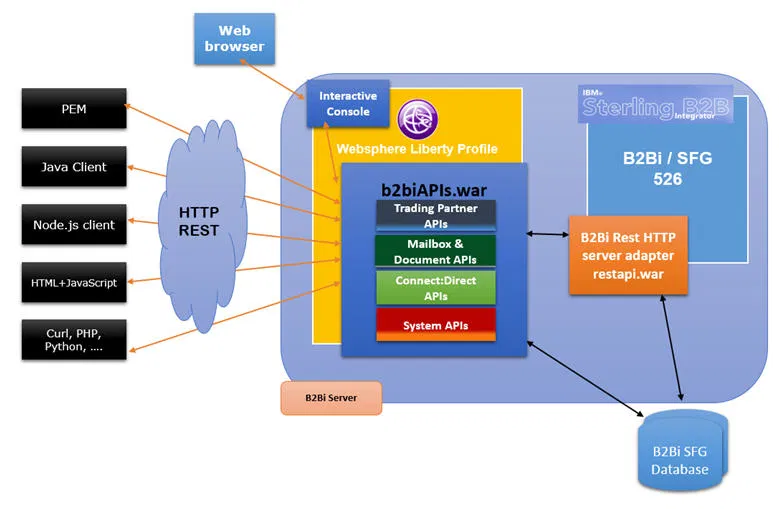
\includegraphics[width=1.0\columnwidth]{images/restapisterling.png}
\end{center}
\caption{Architettura REST API IBM®Sterling B2B Integrator}
\label{fig:apirestste}
\end{figure}






